\pdfoutput=1
\documentclass[twocolumn]{aastex62}
%%\documentclass[]{emulateapj}

%Accepted/received/... %%

\received{xxx}
\revised{yyy}
\accepted{zzz}

%% Command to document which AAS Journal the manuscript was submitted to.
\submitjournal{AAS Journals}

%% Short title/authors

\shorttitle{LXUV History of TRAPPIST-1}
\shortauthors{Fleming et al.}

%% Begin document, title, packages %%
\usepackage{hyperref}
\usepackage{xspace}
\usepackage{graphicx}
\usepackage{amsmath}
\usepackage[caption=false]{subfig}

%% Custom commands
\def\mearth{{\rm\,M_\oplus}}
\def\rearth{{\rm\,R_\oplus}}
\def\msun{{\rm\,M_\odot}}
\def\rsun{{\rm\,R_\odot}}
\def\lsun{{\rm\,L_\odot}}
\def\gsim{~\rlap{$>$}{\lower 1.0ex\hbox{$\sim$}}}
\def\lsim{~\rlap{$<$}{\lower 1.0ex\hbox{$\sim$}}}

\newcommand{\xxx}[1]{{\textbf{#1}}}
\newcommand{\vplanet}[0]{\texttt{VPLanet}\xspace}
\newcommand{\emcee}[0]{\texttt{emcee}\xspace}
\newcommand{\approxposterior}[0]{\texttt{approxposterior}\xspace}
\newcommand{\eqtide}[0]{\texttt{EQTIDE}\xspace}
\newcommand{\stellar}[0]{\texttt{STELLAR}\xspace}
\newcommand{\kepler}[0]{\textit{Kepler}\xspace}
\newcommand{\jwst}[0]{\textit{JWST}\xspace}

%% Begin doc %%
\begin{document}

\title{On The XUV Luminosity Evolution of TRAPPIST-1}

%% AUTHORS %%

%%\correspondingauthor{David P. Fleming}
%%\email{dflemin3@uw.edu}

%%\author[0000-0001-9293-4043]{David P. Fleming}
\author{David P. Fleming}
\affil{Astronomy Department, University of Washington \\
Box 951580, Seattle, WA 98195}
\affil{NASA Astrobiology Institute - Virtual Planetary Laboratory Lead Team, USA}

\author{Rory Barnes}
\affiliation{Astronomy Department, University of Washington \\
Box 951580, Seattle, WA 98195}
\affil{NASA Astrobiology Institute - Virtual Planetary Laboratory Lead Team, USA}

\author{Jake VanderPlas}
\affiliation{Google \\
601 N 34th St, Seattle, WA 98103}

\author{Rodrigo Luger}
\affil{NASA Astrobiology Institute - Virtual Planetary Laboratory Lead Team, USA}
\affiliation{Center for Computational Astrophysics, Flatiron Institute \\
New York, NY 10010}

%% ABSTRACT %%

\begin{abstract}

The James Webb Space Telescope (JWST) is poised to detect and characterize the first terrestrial exoplanet atmosphere in the search for biosignatures \citep{Morley2017,Lustig2019}, but the correct interpretation of those observations is predicated on understanding the system's long-term evolution. Here, we derive probabilistic constraints for TRAPPIST-1's XUV luminosity ($L_{XUV}$) evolution using Markov Chain Monte Carlo (MCMC), accounting for observational uncertainties and correlations between parameters. We apply \approxposterior, a machine learning Python package for Bayesian inference, to compute accurate approximations of posterior distributions and show that this method obtains nearly identical results as traditional MCMC methods, but requires $800\times$ less computational time. We find that there is a $46.2\%$ chance that TRAPPIST-1 is still in the saturated phase today, likely significant atmospheric mass and water loss from its planets.

\end{abstract}

%% Keywords %%

\keywords{}

%% Intro %%

\section{Introduction} \label{sec:intro}

The James Webb Space Telescope (JWST) is poised to detect and characterize the first terrestrial exoplanet atmosphere in the search for biosignatures \citep{Morley2017,Lincowski2018,Lustig2019}, but the correct interpretation of those observations is predicated on understanding the system's long-term evolution, including processes that could impact the planet's habitability, like atmospheric escape \citep{Lammer2003,MurrayClay2009} and water loss \citep{Luger2015}. 

Talk about how XUV is important for atmospheric escape and water loss, e.g. its the major input, and knowing how it changes over time is critical for modeling these planets' atmospheres as a function of time. Then, explain that observations have elucidated how the activity and high-energy radiation of low-mass stars evolves as a function of time. Studies have probed the evolution of the ensemble, but not of individual stars to examine the evolutionary consequences on any planets they may harbor. TRAPPIST-1 is a well-studied nearby M dwarf that hosts 7 transiting exoplants that are prime targets of JWST transmission spectroscopy observations to detect and potentially characterize the first terrestrial exoplanet atmosphere (mention GTO program here). Our theoretical study is timely as we constrain the stellar and XUV evolution of TRAPPIST-1, leaving the water loss modeling, given our constraints, for future work. This study is not just required for TRAPPIST-1, but is required for any planet whose atmospheres we wish to characterize, so it must be computationally-reasonable.

- we constrain the stellar evolution and mass of TRAPPIST-1 using best priors and constraints currently available. we make our posterior distributions available for use with water loss simulations as the FXUV is a core input to such models, be it energy limited or recombination limited, maybe non-thermal escape models as well (look into that). our model and machine learning approach is all open source and documented on github, including a repo for the project itself
- TRAPPIST-1 conference stellar evolution stuff is 1st day, so email invited talks presenters and send them draft and thank them for their work which I use and cite in my own work - adam burgasser and jeff linsky
- from Peacock+2018: "Late-type M stars remain UV active for much longer than their early M counterparts, typically with more variability in the FUV than the NUV (Miles Shkolnik 2017)."

\citet{Newton2017} find that LHalpha, an activity indicator saturates as low Prot/Ro with the cutoff occuring at a similar Ro to other inidicators like Lx

-For low-mass stars in the saturated phase, $L_{X}$ remains a constant fraction of $L_{bol}$ and is observed to cluster around $\log_{10}(L_X/L_{bol}) \approx -3$ \citep{Pizzolato2003,Wright2011,Wright2018}. 

"Although the dynamo processes that drive stellar activity and XUV emission in fully-convective stars have been shown to evolve qualitatively similar to solar-type stars \citep{Wright2016,Wright2018} ..."

- define XUV, what it is, and why it's important

-Introduction about stellar activity for late type stars, what it is like and how late type stars evolve, and finally why it matters for exoplanet habitability, e.g. the XUV flux is a critical parameter for atmospheric escape and water loss, other loss mechanisms scale as FXUV to some power, like energy-limited and recombination-limited escape. In the intro, I explain what saturated and unsaturated phases correspond to physically, and under what conditions they are expected to occur. Argue how this qualitative behavior is observed for both partially and fully-convective stars, e.g. FGK and M dwarfs.

-The saturation ratio shows tentative evidence of increasing with decreasing stellar mass \citep{Wright2011,Jackson2012}, consistent with the observation that later type low-mass stars are more active \citep[e.g.][]{West2008}. 

-"Stellar XUV flux cannot be reliably determined as it is heavily absorbed by the ISM
even for closest stars. However, XUV fluxes are required input parameters for the characterization
of photoionization and photodissociation which are crucial for modeling exoplanetary atmospheric
dynamics and escape (Ribas+2005; Airapetian+2017a; Garcia-Sage+2017; Johnstone+2018; 
Lammer 2018; Glocer+2018). This effort should be combined with empirical and semi-empirical
methods which reconstruct XUV fluxes using FUV/NUV and radiative transfer modeling efforts
(Linsky+2013; France +2016; Peacock+2018; Richey-Yowell+2019)."

-"The XUV stellar spectrum is crucial for understanding the
exoplanetary atmospheric evolution and its impact on habitable worlds as it drives and regulates
atmospheric heating, mass loss and chemistry on Earth-like planets, and thus is critical to the
long-term stability of terrestrial atmospheres."

-"The stellar XUV emission can be reconstructed using empirical and theoretical
approaches. Empirical reconstructions have already provided valuable insights on the level of
ionizing radiation from F, K, G and M dwarfs (Cuntz \& Guinan 2016; France et al. 2016; 2018;
Loyd et al. 2016; Youngblood et al. 2016; 2017). "

-"Lighter species, such as hydrogen, tend to escape more easily through thermal escape, but
strong XUV fluxes can also stimulate the loss of light and heavy ions through ionospheric
outflow and exospheric pick-up by stellar winds (Glocer et al. 2012; Airapetian et al. 2017a;
Kislyakova et al. 2014; Dong et. al. 2017; Lammer et al. 2008; 2018)."

-\citet{Chassefiere1997} for Venusian water loss

We describe our model and statistical methods in $\S$~\ref{sec:model} and $\S$~\ref{sec:mcmc}. We present our results in $\S$~\ref{sec:results}, demonstrate the ability of new machine learning methods to accurately and efficiently reproduce our analysis in $\S$~\ref{sec:approx}, and discuss the implications of our results in $\S$~\ref{sec:discussion}.

\section{Model} \label{sec:model}

We simulate TRAPPIST-1's evolution using the \stellar module in \vplanet \citep{Barnes2019} that performs a bicubic interpolation over mass and age of the \citet{Baraffe2015} stellar evolution tracks. The \citet{Baraffe2015} models, also employed by both \citet{Burgasser2017} and \citet{vanGrootel2018} to constrain TRAPPIST-1's stellar properties, were computed for solar metallicity stars and hence are suitable for TRAPPIST-1 whose [Fe/H] is consistent with solar \citep{Gillon2016}, although \citet{Burgasser2017} argue TRAPPIST-1 has a slightly super-solar metallicity based on isochrone modeling.

The X-ray luminosity, L$_{X}$, evolution of fully-convective stars follows the same broken power law model examined for partially-convective FGK stars \citep{Wright2016,Wright2018}. We assume TRAPPIST-1's L$_{XUV}$ evolution traces that of L$_{X}$ use the model of \citet{Ribas2005},
\begin{align}
\label{eqn:lxuv}
\frac{L_\mathrm{XUV}}{L_\mathrm{bol}} = \left\{
				\begin{array}{lcr}
					f_\mathrm{sat} &\ & t \leq t_\mathrm{sat} \\
					f_\mathrm{sat}\left(\frac{t}{t_\mathrm{sat}}\right)^{-\beta_\mathrm{XUV}} &\ & t > t_\mathrm{sat}
				\end{array}
				\right.,
\end{align}
where $f_{sat}$ is the constant ratio of stellar XUV to bolometric luminosity during the saturated phase, $t_{sat}$ is the duration of the saturated phase, and $\beta_{XUV}$ is the exponent that controls how steeply L$_{XUV}$ decays after saturation.

%% MCMC %%

\section{Markov Chain Monte Carlo} \label{sec:mcmc}

We use \texttt{emcee} \citep{ForemanMackey2013}, a Python implementation of the \citet{Goodman2010} affine-invariant Metropolis-Hastings Markov Chain Monte Carlo (MCMC) sampling algorithm, to infer posterior probability distributions for our model parameters. These parameters comprise the state vector
\begin{equation} \label{eqn:state}
    \textbf{x} = \{m_{\star}, f_{sat}, t_{sat}, \mathrm{age}, \beta_{XUV}\},
\end{equation}
where $m_{\star}$ and age are the stellar mass and age, respectively, and the other parameters are defined by Eqn.~\ref{eqn:lxuv}.  MCMC sampling allows us to derive probability distributions for our model parameters that are conditioned on observations and our understanding on the underlying physics, while accounting for correlations between parameters and their observational uncertainties.  

\subsection{Priors} \label{sec:mcmc:priors}

With only two data points to condition our analysis, TRAPPIST-1's observed $L_{bol}$ and $L_{XUV}$, our prior probability distributions will strongly impact our results. We leverage observations of TRAPPIST-1 and late M dwarfs to assemble the best available empirical constraints to serve as priors for our MCMC analysis and note that these constraints are applicable to any fully-convective M dwarf. We summarize our adopted distributions in Table~\ref{tab:priors}.

Following \citet{vanGrootel2018}, we rely on TRAPPIST-1's luminosity and age to constrain its mass and therefore adopt a uniform prior of $m_{\star} \sim \mathcal{U}(0.07, 0.11)$. We use the empirical age constraint for TRAPPIST-1 derived by \citet{Burgasser2017}, age $\sim \mathcal{N}(7.6, 2.2^2)$ Gyr, as their thorough analysis considered both observations of TRAPPIST-1 and a host of empirical age indicators for ultracool dwarfs. We construct an empirical $f_{sat} = \log_{10}(L_{XUV}/L_{bol})$ distribution from the sample of fully-convective, saturated M dwarfs with observed $L_{X}$ from \citet{Wright2011}. For each star in the \citet{Wright2011} sample, we follow \citet{Wheatley2017} and estimate $L_{XUV}$ as a function of L$_{X}$ using Eqn.~(2) from \citet{Chadney2015}. We find that the distribution is well-approximated by a normal distribution, $f_{sat} \sim \mathcal{N}(-2.92, 0.26^2)$, and we adopt it as our prior.  

The duration of the saturated phase is estimated to be $t_{sat} \approx 100$ Myr for FGK stars \citep{Jackson2012}. Studies of stellar activity of late type stars as a function of stellar age, or its proxy, rotation period, indicate that the activity lifetime, and hence duration of the saturated phase, is likely longer for later-type stars \citep{Shkolnik2014,Wright2011,West2015,GonzalezAlvarez2019}, with fully-convective M dwarfs potentially remaining active for Gyrs, up to the ages of field stars \citep{West2008,Schneider2018}. TRAPPIST-1's high observed L$_{X}$ \citep{Wheatley2017}, short photometric rotation period \citep[3.3 d, ][]{Luger2017}, and low Rossby number \citep[Ro $\approx 0.01$, ][]{Roettenbacher2017} suggest that TRAPPIST-1 is still saturated today \citep{Pizzolato2003,Wright2011,Wright2018,Garraffo2017,GonzalezAlvarez2019}. Both \citet{Roettenbacher2017} and \citet{Morris2018} suggest that the photometrically-determined rotation period is inaccurate, with the latter study proposing that the 3.3 d period corresponds to a characteristic timescale for active regions on the stellar surface, but TRAPPIST-1's $v \sin i = 6$ km s$^{-1}$ \citep{Barnes2014} implies a rotation period of $\approx 1$ d for $i = 90^{\circ}$, providing evidence that TRAPPIST-1's rapid rotation is physical and consistent with saturation.  Given these constraints, we adopt a broad uniform $t_{sat}$ prior distribution over $0.1 - 12$ Gyr.

In the unsaturated phase, $L_{X}$, and hence $L_{XUV}$, decay exponentially with powerlaw slope $\beta_{XUV}$ \citep{Ribas2005}. \citet{Jackson2012} find that $\beta_{XUV}$ does not significantly vary with stellar mass in their sample of FGK stars. \citet{Wright2016} found that the X-ray evolution of fully-convective stars is qualitatively similar to that of partially-convective FGK stars, therefore, we adopt the distribution of late K dwarfs from the \citet{Jackson2012} sample as our prior, $\beta_{XUV} \sim \mathcal{N}(-1.18, 0.31^2)$.

\begin{deluxetable}{lcc}
\tabletypesize{\small}
\tablecaption{Prior Distributions \label{tab:priors}}
\tablewidth{0pt}
\tablehead{
\colhead{Parameter [units]} & \colhead{Prior} & \colhead{Notes}
}
\startdata
$m_\star$ [$M_{\odot}$] & $\mathcal{U}(0.07, 0.11)$ & -- \\  
$f_{sat}$ & $\mathcal{N}(-2.92, 0.26^2)$ & \citet{Wright2011}  \\
$t_{sat}$ [Gyr] & $\mathcal{U}(0.1, 12)$ & -- \\
age [Gyr] & $\mathcal{N}(7.6, 2.2^2)$ & \citet{Burgasser2017} \\
$\beta_{XUV}$ & $\mathcal{N}(-1.18, 0.31^2)$ & \citet{Jackson2012}
\enddata \vspace*{0.1in}
\end{deluxetable}

\subsection{Likelihood Function and Convergence}

We further condition our analysis on TRAPPIST-1's observed bolometric luminosity, $L_{bol} = 5.22 \pm{0.19} \times 10^{-4} \ L_{\odot}$ \citep{vanGrootel2018}, and $L_{XUV}/L_{bol}$ \citep{Wheatley2017}. We convolve the \citet{vanGrootel2018} $L_{bol}$ measurement with the $L_{XUV}/L_{bol}$ constraints from \citet{Wheatley2017} and find $L_{XUV} = 3.9 \pm{0.5} \times 10^{-7} \ L_{\odot}$.

For a given state vector \textbf{x}, we define our loglikelihood function as
\small
\begin{equation} \label{eqn:lnlike}
\begin{split}
    \ln \mathcal{L} \propto & -\frac{1}{2} \left[ \frac{(L_{bol} - L_{bol}(\textbf{x}))^2}{\sigma_{L_{bol}}^2} + \frac{(L_{XUV} - L_{XUV}(\textbf{x}))^2}{\sigma_{L_{XUV}}^2} \right] \\
    & + \ln \mathrm{Prior}(\textbf{x})
\end{split}
\end{equation}
\normalsize
where $L_{bol}$, $L_{XUV}$ and $L_{bol}(\textbf{x})$, $L_{XUV}(\textbf{x})$ are the observed values and \vplanet outputs given \textbf{x}, respectively, $\sigma_{L_{bol}}$ and $\sigma_{L_{XUV}}$ are the observational uncertainties, and $\ln \mathrm{Prior}(\textbf{x})$ is the prior probability. 

We run our MCMC with 100 parallel chains for 10,000 iterations, initializing each chain by randomly sampling each element of \textbf{x} from their respective prior distributions. Each step of the MCMC chain, \vplanet takes \textbf{x} as input and simulates TRAPPIST-1's evolution up to its age, predicting $L_{bol}$ and $L_{XUV}$ to evaluate the likelihood function. We discard the first 500 iterations as burn-in and assess the convergence of our MCMC chains by computing the integrated autocorrelation length and acceptance fraction for each chain. We find a mean acceptance fraction of 0.45 and a minimum and mean number of iterations per integrated autocorrelation length of 75 and 110, respectively, indicating that our chains have converged \citep{ForemanMackey2013}.

%% Results %%

\section{Results} \label{sec:results}

In Fig.~\ref{fig:corner}, we display the posterior probability distributions for our model parameters derived by our MCMC analysis, adopting the median values of the marginal distributions as our best-fit solutions and derive the lower and upper uncertainties using the 16th and 84th percentiles, respectively. TRAPPIST-1 likely maintained a large $L_{XUV}$ throughout its lifetime, with our MCMC analysis uncovering strong correlations between the model parameters that control this evolution. We find TRAPPIST-1's $f_{sat} = -3.05^{+0.24}_{-.10}$ and $t_{sat} = 6.85^{+3.43}_{-3.15}$ Gyr, both deviating significantly from their priors and consistent with observed $L_{XUV}/L_{bol}$ and long activity lifetimes of late M dwarfs \citep{West2008,Wright2018}. The long upper-tail in the marginalized $f_{sat}$ distribution arises from the combination of the degeneracy between $f_{sat}$ and $t_{sat}$ and from our strong empirical $f_{sat}$ prior that disfavors $f_{sat} \gsim -2.7$. To match TRAPPIST-1's observed $L_{XUV}$, larger values of $f_{sat}$, e.g. large initial $L_{XUV}$, require shorter $t_{sat}$, and hence earlier powerlaw $L_{XUV}$ decay during the unsaturated phase, and vice-versa. We infer that there is a $42.6\%$ chance that TRAPPIST-1 is still in the saturated phase today, i.e. P$(t_{sat} \geq \mathrm{ age } | \mathrm{data}) \approx 0.426$. Our analysis strongly disfavors short saturation timescales, with only a $0.4\%$ chance that $t_{sat} \leq 1$ Gyr, the saturation timescale adopted by \citet{Luger2015} in their analysis of water loss from exoplanets orbiting in the habitable zone of late M dwarfs. These constraints imply that TRAPPIST-1 has likely maintained a high $L_{XUV}$ throughout its lifetime, potentially driving extreme water loss from its planets.

\begin{figure*}[t]
\centering
	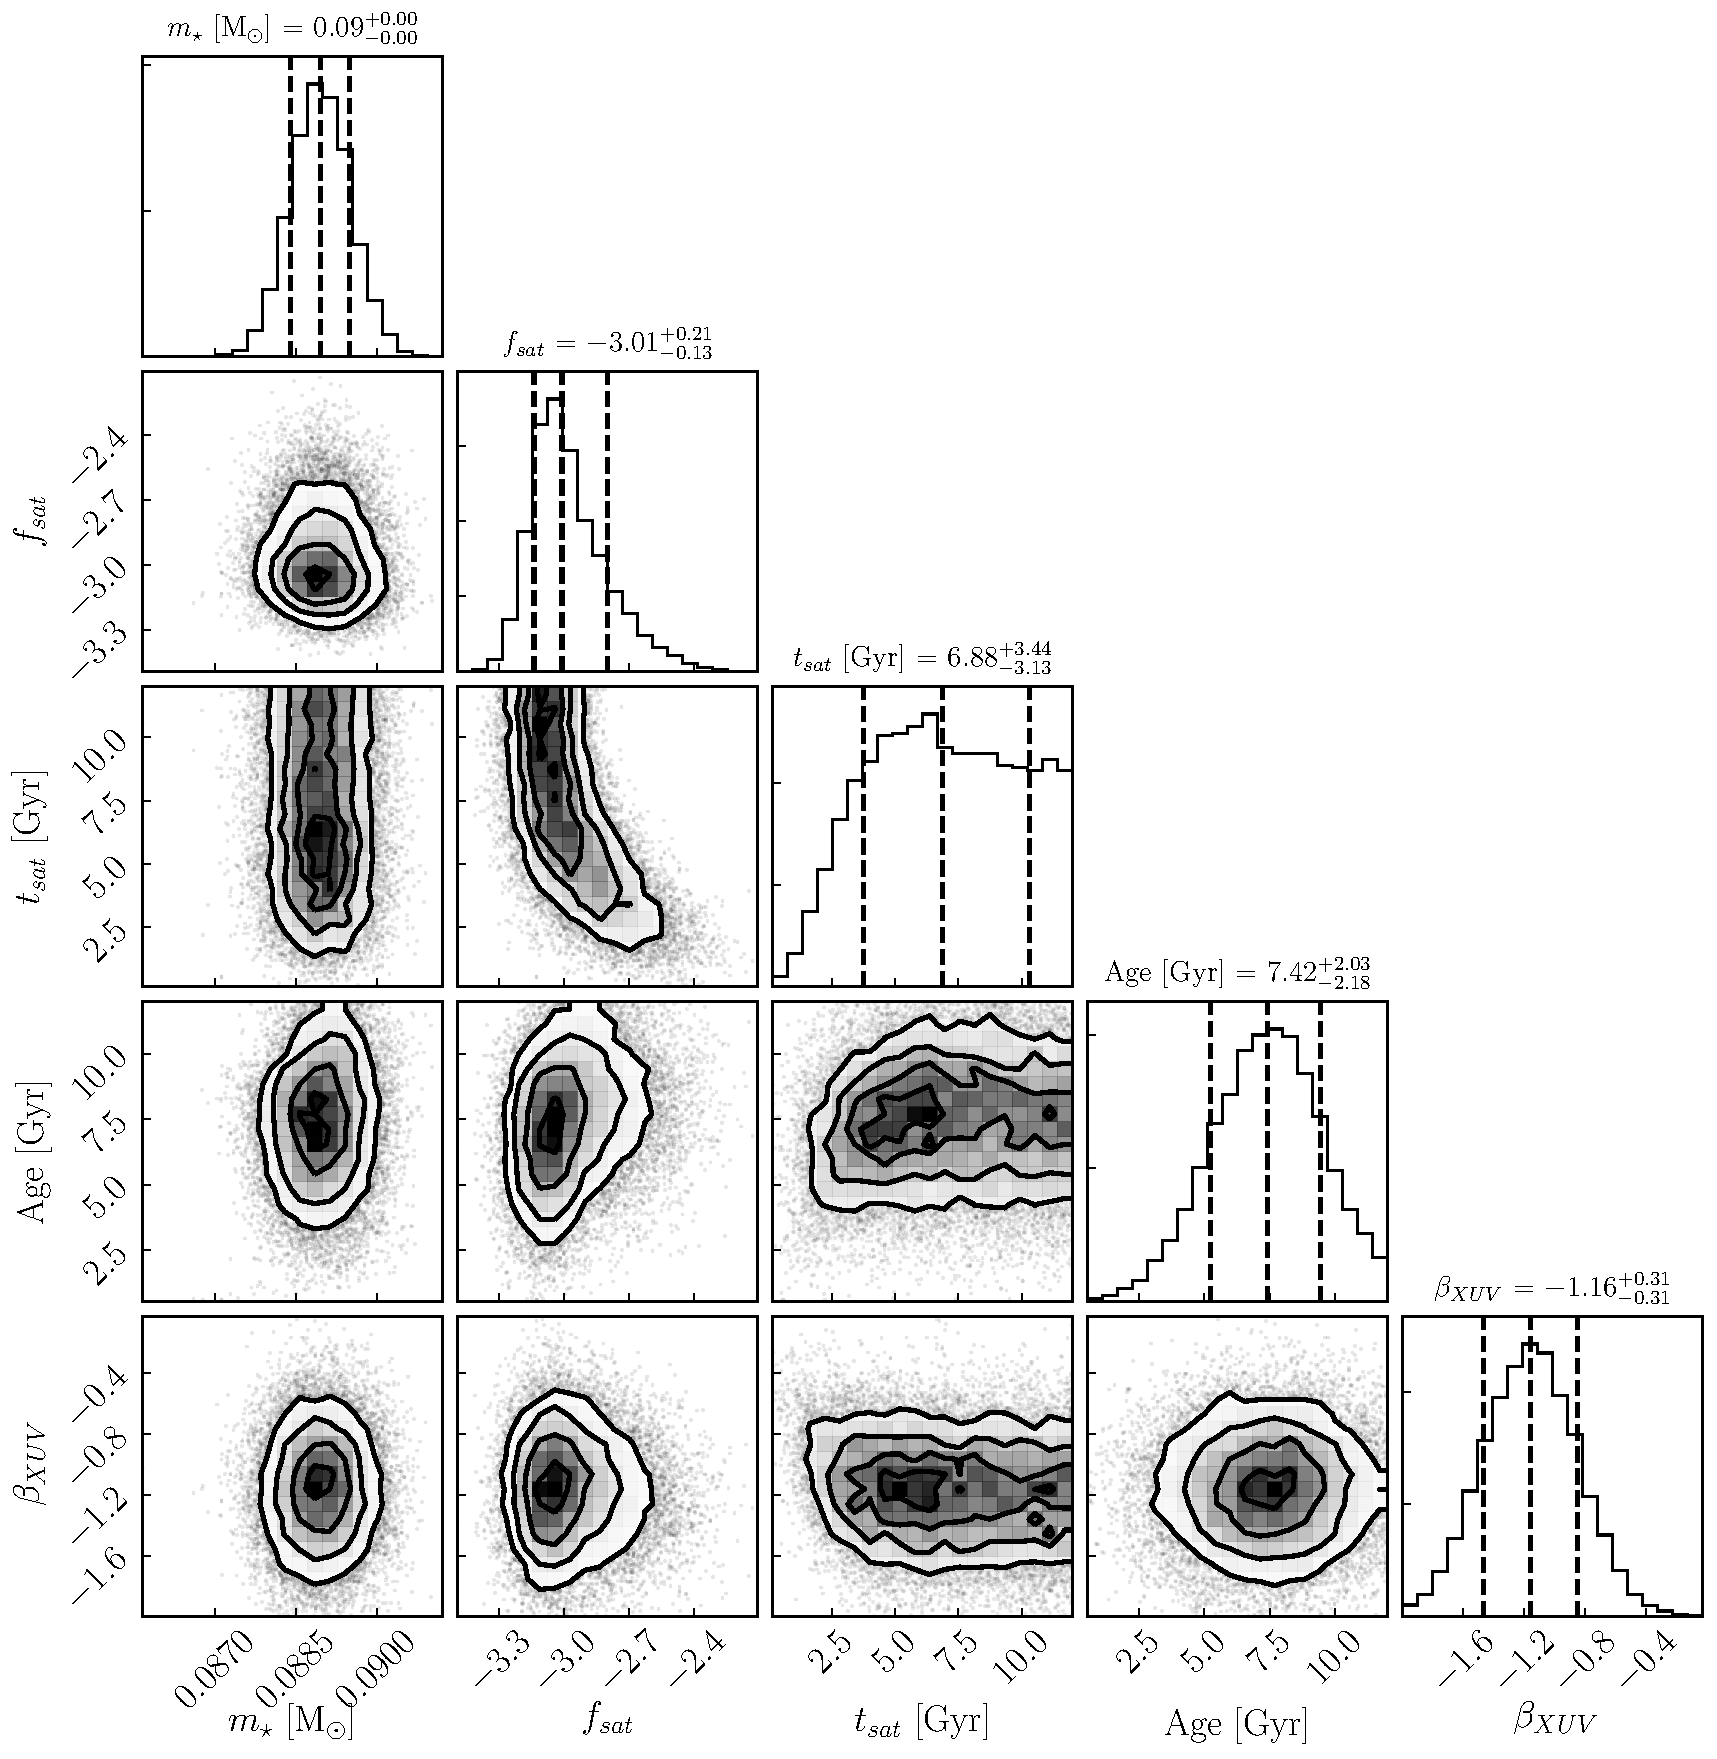
\includegraphics[width=0.75\textwidth]{../Analysis/Corner/trappist1Corner.pdf}
   \caption{Joint and marginal posterior probability distributions for the TRAPPIST-1 stellar parameters given in Eqn.~(\ref{eqn:state}) made using \texttt{corner} \citep{ForemanMackey2016}. The black vertical dashed lines on the marginalized distributions indicate the median values and lower and upper uncertainties from the 16th and 84th percentiles, respectively. From the posterior, we infer that there is a $42.6\%$ chance that TRAPPIST-1 is still in the saturated phase today, potentially driving significant water loss and atmospheric escape from its planets.}%
    \label{fig:corner}%
\end{figure*}

We constrain TRAPPIST-1's mass to $m_{\star} = 0.089 \pm{0.0006}$ M$_{\odot}$, identical to the \citet{vanGrootel2018} constraint. Our marginalized age and $\beta_{XUV}$ posterior distributions reflect their prior distributions as for the former, $L_{bol}$ is not sufficient to further constrain TRAPPIST-1's age beyond our adopted prior since the luminosities of M dwarfs do not significantly change during the main sequence \citep{Baraffe2015}. We do not constrain $\beta_{XUV}$ past out prior because our model prefers to exploit the degeneracy between $f_{sat}$ and $t_{sat}$ to match TRAPPIST-1's observed $L_{XUV}$, instead of varying the slope of the $L_{XUV}$ decay during the unsaturated phase, likely because TRAPPIST-1 could still be saturated, rendering $\beta_{XUV}$ unnecessary to model its $L_{XUV}$ evolution. Age and $\beta_{XUV}$ weakly correlate with $f_{sat}$, both requiring a narrow spread of $f_{sat} \approx -3.05$ for young ages and steeper $\beta_{XUV}$. $\beta_{XUV}$ and $t_{sat}$ are uncorrelated, except at short $t_{sat}$ where steep $\beta_{XUV}$ are disfavored as this evolution would underpredict $L_{XUV}$.

\subsection{TRAPPIST-1's Evolutionary History}

Here we consider plausible stellar evolutionary histories for TRAPPIST-1, conditioned on observations, by evolving 100 samples from the posterior distribution using \vplanet. We plot the evolution of TRAPPIST-1's $L_{bol}$, $L_{XUV}$, and radius in Fig.~\ref{fig:evol} and compare our models to the measured values. 

\begin{figure*}[t]
	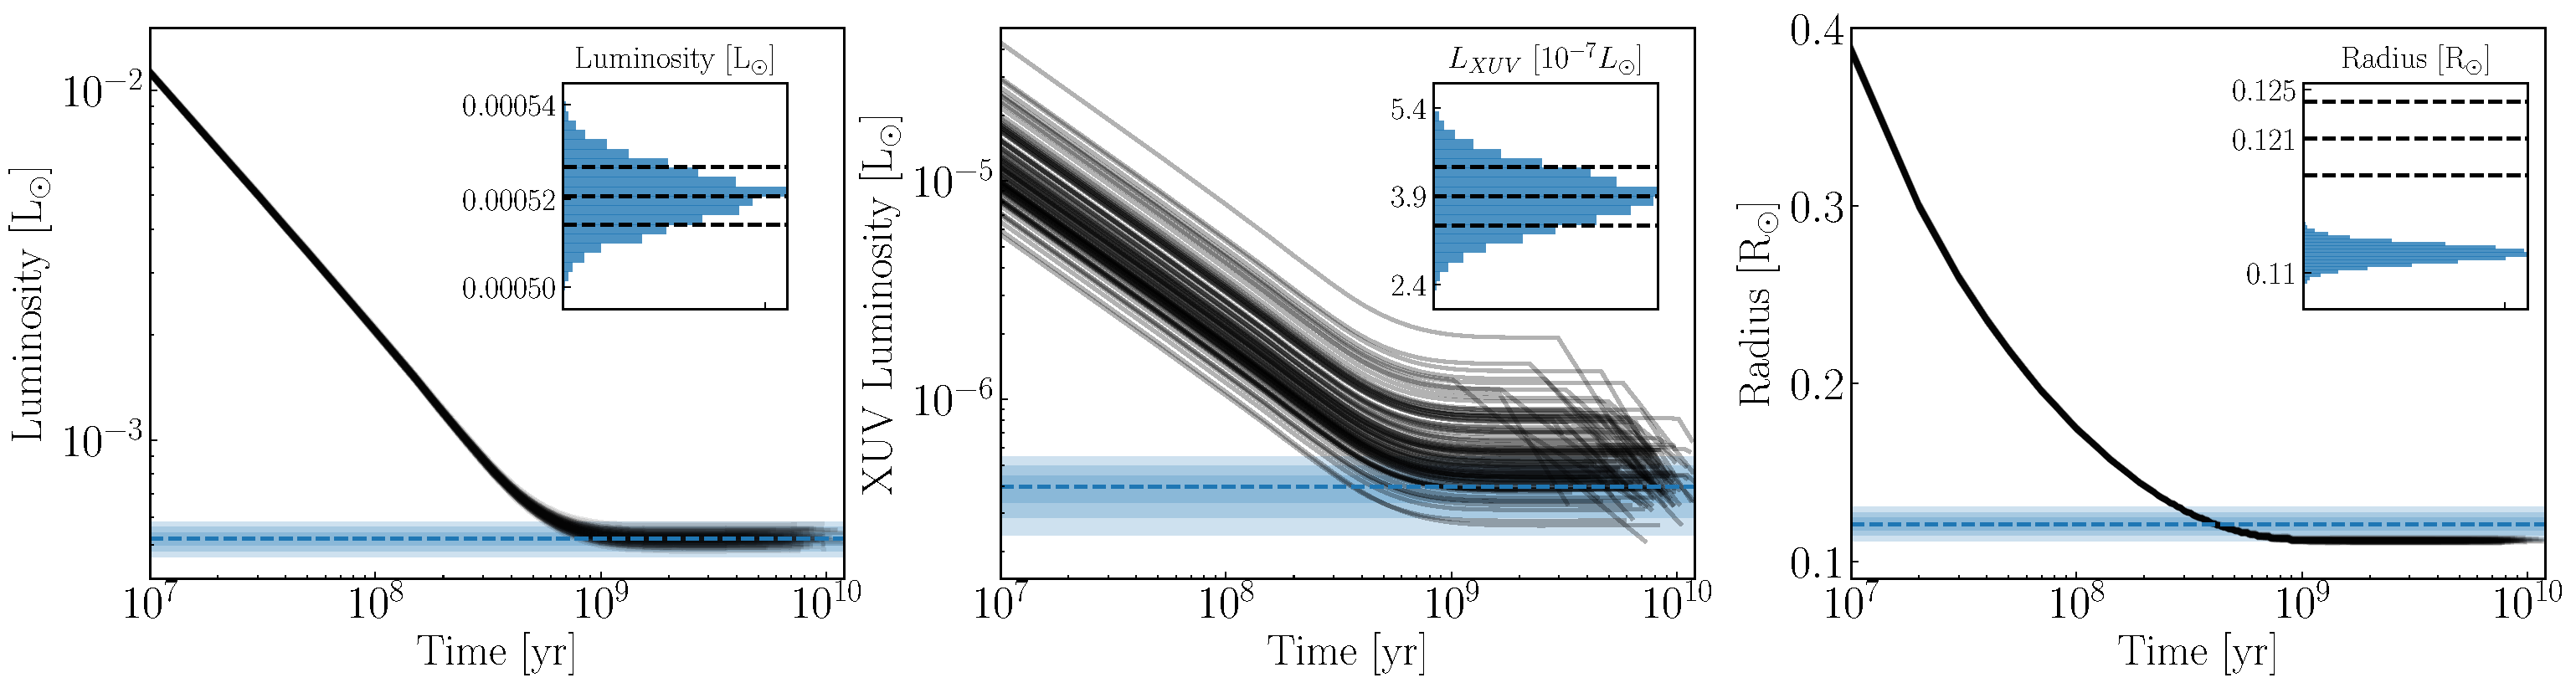
\includegraphics[width=\textwidth]{../Analysis/Evol/trappist1Evol.pdf}
   \caption{Plausible evolutionary histories of TRAPPIST-1's bolometric luminosity (left), XUV luminosity (center), and radius (right) using 100 samples drawn from the posterior distribution and simulated with \vplanet. In each panel, the blue shaded regions display the 1, 2, and 3 $\sigma$ the observational uncertainties. The insets display the marginalized distributions (black) evaluated at the age of the system, with the blue dashed lines indicating the observed value and +/- 1 $\sigma$ uncertainties. The radius and bolometric luminosity constraints are adopted from \citet{vanGrootel2018}, and the L$_{XUV}$ constraint is adapted from \citet{Wheatley2017}.}%
    \label{fig:evol}%
\end{figure*}

Since TRAPPIST-1 could still be saturated today, its planetary system has likely experienced a persistent extreme XUV environment, potentially driving massive water loss \citep[][Fleming et al., in prep]{Luger2015,Bolmont2017,Bourrier2017a}. For example, from our posterior distributions, we infer that TRAPPIST-1b, if its remained near its current semi-major axis after migration halted \citep{Luger2017}, likely received from $XXX \times F_{XUV, \oplus}$ over TRAPPIST-1's pre-main sequence lifetime. TRAPPIST-1's $L_{XUV}$ evolution tracks $L_{bol}$, both decreasing by a factor of ${\sim}40$ along the pre-main sequence before stabilizing on the main sequence, with ${\sim}60\%$ of $L_{XUV}$ evolutions entering the unsaturated powerlaw decay at late times near the age of the system. 

TRAPPIST-1's radius likely shrank by roughly a factor of 4 along the pre-main sequence, with our posterior present-day radius $R_{\star} = 0.11 \pm{0.0008} \ R_{\odot}$. Our posterior radius is ${\sim} 8\%$ smaller than the \citet{vanGrootel2018} constraint, $R_{\star} = 0.121 \pm {0.003} \ R_{\odot}$, that was computed from their inferred mass and TRAPPIST-1's density \citep{Delrez2018}. This difference arises from the likely underprediction of TRAPPIST-1's radius by the \citet{Baraffe2015} models, consistent with stellar evolution models often underestimating the radii of late M dwarfs \citep{Reid2005,Spada2013,Jackson2019}, and suggests that TRAPPIST-1 might have super-solar metallicity \citep{Burgasser2017,vanGrootel2018} to account for its inflated radius. If we instead follow \citet{vanGrootel2018} and compute the radius from our marginalized stellar mass posterior distribution and the \citet{Delrez2018} density constraint, we obtain $R_{\star} = 0.12 \pm{0.002} \ R_{\odot}$, in agreement with the \citet{vanGrootel2018} constraint.

%% approxposterior %%

\section{Inference Using \approxposterior} \label{sec:approx}

The methods presented in this work can be applied to any late-type star to constrain its $L_{XUV}$ history, given suitable priors and observational constraints. Characterizing these XUV fluxes is critical for studies of atmospheric escape, water-loss, and atmospheric photochemistry on exoplanets \citep[e.g.][]{Lammer2003,Ribas2005,MurrayClay2009,Luger2015,Airapetian2019}. Our MCMC analysis, however, required 3,700 core hours on the University of Washington Hyak supercomputer. Assuming similar convergence properties, repeating this analysis for even a modest sample of 30 stars would require~${\sim} 110,000$ core-hours, a non-trivial computational expense. 

% Extra
%If using a slower model than ours, perhaps one that models stellar evolution by interpolating tracks over mass, age, and metallicity to additionally constrain [Fe/H], or if testing alternate models of $L_{XUV}$ evolution for model comparisons, the computational expense will grow, exacerbating this issue.

We apply \approxposterior\footnote{\approxposterior is publicly available on \href{https://github.com/dflemin3/approxposterior}{GitHub}.}, an open source Python machine learning package, to compute an accurate approximation to the true MCMC-derived posterior distribution for TRAPPIST-1's XUV evolution, while minimizing the computational cost \citep{FlemingVanderPlas2018}. In the MCMC analysis, the main computational cost is incurred by running a $10$s \vplanet simulation each MCMC step to evaluate the likelihood, requiring ${\sim}1,000,000$ simulations in total for the full MCMC. \approxposterior, an implementation of the ``Bayesian Active Learning for Posterior Estimation" (BAPE) algorithm of \citet{Kandasamy2015}, trains a Gaussian process \citep[GP, ][]{Rasmussen2006} surrogate for the likelihood evaluation, learning on the results of \vplanet simulations. The GP is then used within an MCMC sampling algorithm to obtain the posterior distribution. Following \citet{Kandasamy2015}, \approxposterior iteratively improves the GP's predictive ability by identifing high-likelihood regions in parameter space where the GP predictions are uncertain. \approxposterior then evaluates \vplanet in those regions to supplement the training set, improving the GP's predictive ability in the relevant regions of parameter space, while minimizing the number of forward model evaluations required for suitable predictive accuracy. Similar techniques using a GP surrogate model have been shown to rapidly and accurately infer \citep[e.g.][]{Bird2019,Rogers2019,Takhtaganov2019} and reconstruct \citep{McClintock2019} Bayesian posterior distributions for computationally-expensive cosmology studies.

To model the covariance between points, we use a squared exponential kernel,
\begin{equation} \label{eqn:kernel}
k(x_i, x_j) = \exp \left( - \frac{(x_i - x_j)^2}{2l^2} \right),
\end{equation}
where $x_i$ and $x_j$ are two arbitrary points in parameter space and $l$ is hyperparameter that controls the scale length of the correlations. We assume correlations in each dimension have different scale lengths and fit for each $l$ by optimizing the GP's marginal likelihood of the training set data using the Nelder-Mead algorithm \citep{Nelder1965}, randomly restarting this optimization 25 times to mitigate the influence of local extrema. We run \approxposterior for 10 iterations, training the GP on an initial training set of 250 \vplanet simulations distributed over parameter space as a Latin hypercube following \citet{Bird2019}. Each iteration, \approxposterior selects 100 new training points, alternating between the \citet{Kandasamy2015} and \citet{Wang2017} selection criterion and running \vplanet at each point for a total of 1,250 training points. 

We use \approxposterior within \emcee to obtain the approximate posterior distribution depicted in Fig.~\ref{fig:approx}.

\begin{figure*}[t]
\centering
	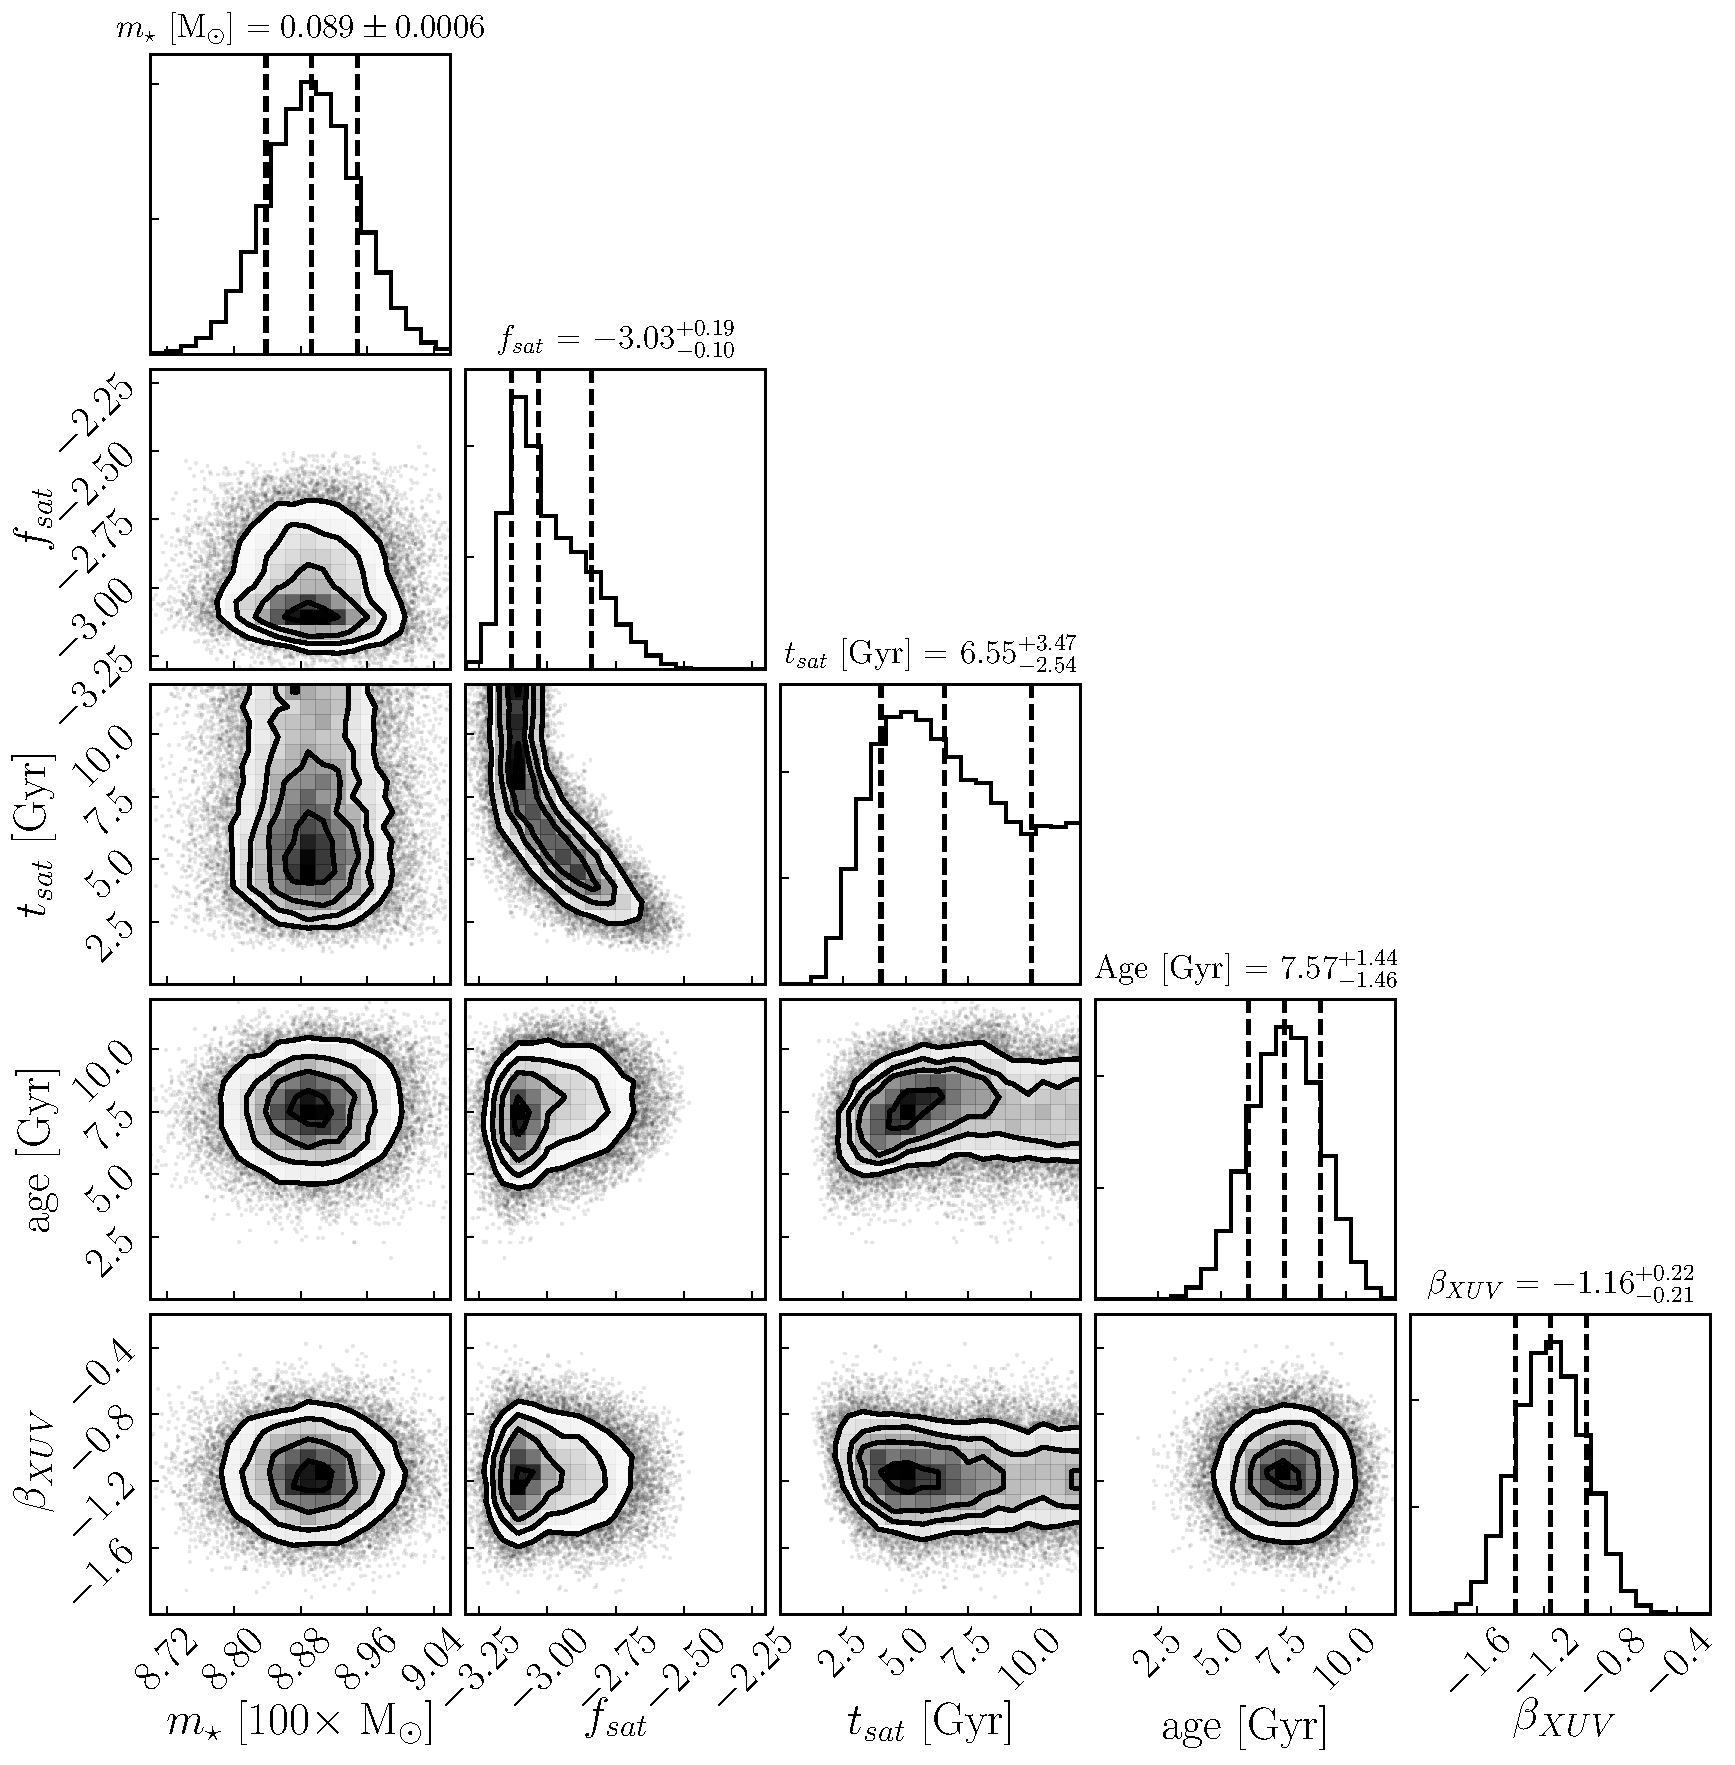
\includegraphics[width=0.75\textwidth]{../Analysis/Approx/apCorner.pdf}
   \caption{Same format as Fig.~\ref{fig:corner}, but creating used \approxposterior.}%
    \label{fig:approx}%
\end{figure*}

\approxposterior uses significantly less computational resources than traditional MCMC methods, requiring $800\times$ fewer \vplanet simulations to build its training set and requiring only 11 core hours to complete, a factor of $336\times$ faster than our MCMC approach. 

\begin{deluxetable}{lcc}
\caption{Parameter Constraints} \label{tab:constraints}
\tabletypesize{\small}
\tablewidth{0pt}
\tablehead{
\colhead{Parameter [units]} & \colhead{MCMC} & \colhead{\approxposterior}
}
\startdata
$m_\star$ [$M_{\odot}$] & $0.089 \pm{0.0006}$ & $0.089 \pm{0.0006}$ \\  
$f_{sat}$ & $-3.05^{+0.24}_{-0.10}$ & $-3.03^{+0.19}_{-0.10}$,  \\
$t_{sat}$ [Gyr] & $6.85^{+3.43}_{-3.15}$ & $6.55^{+3.47}_{-2.54}$ \\
age [Gyr] & $7.44^{+2.04}_{-2.13}$ & $7.57^{+1.44}_{-1.46}$ \\
$\beta_{XUV}$ & $-1.16^{+0.31}_{-0.30}$ & $-1.16^{+0.22}_{-0.21}$
\enddata \vspace*{0.1in}
\tablecomments{Best fit values and uncertainties are derived using the medians, $16^{th}$, and $84^{th}$ percentiles from the marginalized posterior distributions, respectively.}
\end{deluxetable}

%% Discussion %%

\section{Discussion and Conclusions} \label{sec:discussion}

The TRAPPIST-1 planets are prime targets for atmospheric detection and characterization via JWST transmission spectroscopy observations (TRAPPIST-1 b is the target of an approved \jwst~GTO program, Proposal \#1279, for example). Here, we modelled the stellar and $L_{XUV}$ evolution of TRAPPIST-1 to constrain the evolving XUV environment of its planetary system as the correct interpretation of those observations is predicated on understanding the system's long-term evolution and these fluxes are the principal drivers of atmospheric escape and photochemistry. Using MCMC, we derived probabilistic constraints for TRAPPIST-1's stellar and $L_{XUV}$ evolution, inferring that TRAPPIST-1 maintained high $L_{XUV}/L_{bol} \approx 10^{-3}$ throughout its lifetime, with a $42.6\%$ chance that TRAPPIST-1 is still in the saturated regime today.  We demonstrated that using the machine learning Python package, \approxposterior \citep{FlemingVanderPlas2018}, significantly reduces the computational expense of deriving the posterior distribution, requiring $800\times$ fewer \vplanet simulations and was a factor of $336\times$ faster than traditional MCMC approaches, a massive reduction in compute time that allows us to scale these methods to a large sample of late-type dwarfs. The approximate posterior distributions derived by \approxposterior accurately reproduced the non-trivial parameter correlations uncovered by our MCMC analysis and the approximate marginalized constraints were in good agreement with those derived by MCMC. When combined with \approxposterior, our method can efficiently be used to constrain the long-term stellar and $L_{XUV}$ evolution of $100$s of late-type stars to constrain stellar activity histories or to model the atmospheric mass-loss or photochemistry of any planets they may harbor, a key requirement for interpreting observations of exoplanetary atmospheres.

In a subsequent work (Fleming et al., in prep), we examine how our TRAPPIST-1 XUV constraints drive water loss from the TRAPPIST-1 planets.

suggesting that ultracool dwarfs can sustain large XUV luminosities for Gyrs. Our results suggest that the atmospheric erosion of the TRAPPIST-1 planets was likely significant in the past and could be on-going, potentially driving extreme water loss \citep{Bolmont2017,Bourrier2017a}.

%% ACKNOWLEDGEMENTS %%
\acknowledgments
This work was facilitated though the use of advanced computational, storage, and networking infrastructure provided by the Hyak supercomputer system and funded by the Student Technology Fund at the University of Washington. DPF was supported by NASA Headquarters under the NASA Earth and Space Science Fellowship Program - Grant 80NSSC17K0482.  RB acknowledges support from the NASA Astrobiology Institute's Virtual Planetary Laboratory under Cooperative Agreement number NNA13AA93A.

%% SOFTWARE %%
\software{\approxposterior: \citet{FlemingVanderPlas2018}, \texttt{corner}: \citet{ForemanMackey2016}, \texttt{emcee}: \citet{ForemanMackey2013}, \texttt{matplotlib}: \citet{Hunter2007}, \texttt{numpy}: \citet{vanderWalt2011}, \vplanet: \citet{Barnes2019}} 

%% BIBLIOGRAPHY %%

\bibliography{trappist}

% End of file
\end{document}